\chapter{Thermodynamik}
\section{Thermodynamik und Allgemeine\\Definitionen}
\subsection{1}
\begin{myfrag}
Was ist ein Makrozustand und ein Mikrozustand?
Was sind Zustandsgrößen?
\end{myfrag} \qquad \newline
Makrozustand 
\begin{itemize}
\item Beschreibt ein System mit vielen Freiheitsgraden durch einige wenige Zustandsvariablen (z.B. T,p,V,..) viele Teilchen, gemittelte Parameter besteht aus Mikrozuständen mit Wahrscheinlichkeiten.
\end{itemize}
Mikrozustand:
\begin{itemize}
\item Vollständige mikroskopische Beschreibung eines Systems. Punkt im Phasenraum des Systems, Orb- und Geschwindigkeitsvektor pro Teilchen
\end{itemize}
Zustandsgrößen:
\begin{itemize}
\item Sind thermodynamische Variablen, die einen Zustand eindeutig beschreiben (und Umgekehrt) z.B. T,p,V,E keine Zustandsgrößen sind Q, W. Zustandsgrößen haben vollständige Differentiale für reversible Prozesse
\end{itemize}
\subsection{2}
\begin{myfrag}
Was ist ein vollständiges Differential? Was ist ein integrierender Faktor?
In welchem Zusammenhang werden diese Konzepte in der
Thermodynamik benötigt (gebe Beispiele)?
\end{myfrag} \qquad \newline
Ein Differential $dA = a(x,y)dx+b(x,y)dy$ ist vollständig, falls eine Funktion $A(x,y)$ existiert, so dass:
\begin{compactenum}[(i)]
\item $a(x,y) = \left(\dfrac{\partial A}{\partial x} \right) _y $ und $b(x,y) = \left( \dfrac{\partial A}{\partial y} \right) _x $
\item $\oint_\gamma dA = 0 $
\item $\int_a^b dA $ ist wegunabhängig
\item $\left(\dfrac{\partial a}{\partial y} \right) _x = \left(\dfrac{\partial b}{\partial x} \right) _y $
Integrierender Faktor zu einem unvollständigem Differential $\partial B$ ist eine Funktion $g(x,y)$ s.d. $dA = g(x,y)\partial B $ vollständig ist. \newline
$ dV = \dfrac{\delta W}{p} \qquad dS = \dfrac{\delta Q}{T}$ \quad vollständig für reversible Prozesse 
$ dE = \delta Q + \delta W$
\end{compactenum}
\subsection{3}
\begin{myfrag}
Was besagen der Nullte und der Erste Hauptsatz der Thermodynamik?
\end{myfrag} \quad \\
Nullter Hauptsatz:
\begin{itemize}
\item 2 Systeme sind im thermischen Gleichgewicht, wenn kein Wärmeübertrag bei kontakt stattfindet d.h. sie haben die gleiche Temperatur.
$\rightarrow$ impliziert existenz von Temperatur
\end{itemize}
Erster Hauptsatz:
\begin{itemize}
\item Die Energie ist eine Zustandsgröße, d.h. $dE= \delta Q + \delta W $ ist vollständig. $ \delta W = -Fdx = -pdV$.\\
Die Energie bleibt also erhalten.
\end{itemize}
\subsection{4}
\begin{myfrag}
Was ist eine generalisierte Kraft? Gebe ein Beispiel!
\end{myfrag} \quad \\
Eine generalisierte Kraft $F_\alpha$ , konjugiert zu einer Variablen $\alpha$, ist definiert durch: \\[2ex]
$F_\alpha = - \left( \dfrac{\partial E}{\partial \alpha} \right) _{S,andere \alpha}\qquad $ Druck
$p = -\left(\dfrac{\partial E}{\partial V} \right) _S \qquad
$ Magnetisierung
$m= -\left(\dfrac{\partial E}{\partial B} \right) _S $
\subsection{5}
\begin{myfrag}
Wie ist die Entropie in der Thermodynamik definiert? Was sind
reversible Prozesse?
\end{myfrag}
Die Entropie ist das Integral des vollständigen Differentials $dS = \dfrac{\delta Q}{T}$ \\"vollständig für reversible Prozesse" \\[2ex]
Reversibler Prozess:
\begin{itemize}
\item Ein reversibler Prozess ist eine Zustandsänderung eines Körpers, der jederzeit wieder umgekehrt ablaufen kann.
\item Zeitlich invariant. 
\item Zu jedem Zeitpunkt im Gleichgewicht ablaufend.
\ Aneinanderreihung von quasistatischen Zuständen (zeitlich umkehrbar)
\end{itemize} 

\subsection{6}
\begin{myfrag}
Was besagt der Zweite Hauptsatz der Thermodynamik?
\end{myfrag} \quad \\
Zweiter Hauptsatz (nach Clausius Version 1850): \\[2ex]
\begin{wrapfigure}{r}{0.3\textwidth}
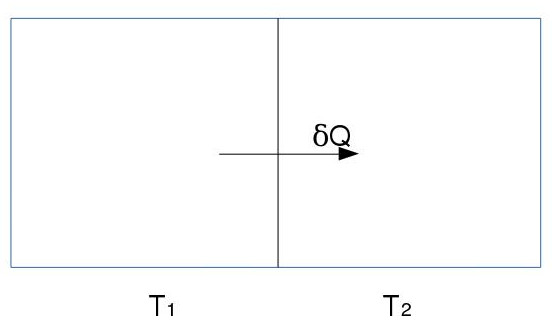
\includegraphics[width=5cm]{Bilder/Frage6.jpg} 
\end{wrapfigure}
Wärme $\delta Q$ geht spontan nur von einer höheren zu einer tieferen Temperatur. \\
$dS_1 = - \dfrac{\delta Q}{T_1} \\
dS_2 = \dfrac{\delta Q}{T_2} \\
\Delta S = dS_1 + dS_2 = \delta Q ( \dfrac{1}{T_2} -\dfrac{1}{T_1}) > 0$ \\
$\rightarrow $ Entropie erhöht sich $\rightarrow  \Delta S \geq \int_a^b \dfrac{\delta Q}{T} $ wobei Gleichgewicht bei reversiblen Prozessen.
\subsection{7}
\begin{myfrag}
Gebe die thermodynamischen Definitionen für die Freie Energie F, die
Enthalpie H, die Freie Enthalpie G und das Grosskanonische Potential $\Phi $
an. Was sind jeweils die entsprechenden Differentiale? Wie können
thermodynamische Größen und generalisierte Kräfte mit den
thermodynamischen Potentialen berechnet werden?
\end{myfrag} \quad \\
Freie Energie : $F(T,V,N) = E-TS \quad dF = -SdT -pdV+\mu dN$ \\
Enthalpie : $ H(S;p,N)=E-TS+pV \quad dH = TdS +Vdp+\mu dN$ \\
Freie Enthalpie : $ G(T;p;N)=E_TS+pV \quad dG=-SdT+Vdp+\mu dN$ \\
Großkanonisches Potential : $\Phi(T,V,\mu ) = F-\mu N \quad d \Phi = -SdT-pdV-Nd \mu $ \\[2ex]

$ F_\alpha = - \left( \dfrac{\partial E}{\partial \alpha }\right) _{S,andere \alpha} \quad a(x,y)= \left( \dfrac{\partial A}{\partial x}\right) _y \qquad b(x,y) = \left( \dfrac{\partial A}{\partial y }\right) _x$
\subsection{8}
\begin{myfrag}
Was ist eine Legendre-Transformation?
\end{myfrag}
Legendre Transformation $H= \vec{p}\vec{q}-L(\dot{\vec{q}},q)=H(p,\vec{q} )$ \\
Eine Legendre Transformation bildet aus einer Funktion $A(x,y)$ mit $ dA= a(x,y)dx +b(x,y)dy$ eine neue Funktion $B=A-ax$ mit Differential $ dB = dA - adx -xda = bdy -xda$ Das Integral ist eine Funktion von $B(a,y)$
\subsection{9}
\begin{myfrag}
Was sind intensive und extensive thermodynamische Variablen? Gebe
Beispiele.
\end{myfrag} \quad \newline
Intensive Größen 
\begin{itemize}
\item Sind unabhängig vom Ausmaß $\alpha $ des Systems (z.B. p,T,B,$\mu $)
\end{itemize}
Extensive Größen
\begin{itemize}
\item sind proportional zum Ausmaß $\alpha (E,F,G,H, \Phi , m, N, V)$
\end{itemize}
Wie erkennt man den unterschied? Man nehme zwei identische Systeme und Trenne diese mit einer Trennwand. Entfernt man die Wand dann bleiben alle intensive Größen gleich und die extensiven ändern sich.